\chapter{\IfLanguageName{dutch}{Stand van zaken}{State of the art}}%
\label{ch:stand-van-zaken}

% Tip: Begin elk hoofdstuk met een paragraaf inleiding die beschrijft hoe
% dit hoofdstuk past binnen het geheel van de bachelorproef. Geef in het
% bijzonder aan wat de link is met het vorige en volgende hoofdstuk.

% Pas na deze inleidende paragraaf komt de eerste sectiehoofding.

%Dit hoofdstuk bevat je literatuurstudie. De inhoud gaat verder op de inleiding, maar zal het onderwerp van de bachelorproef *diepgaand* uitspitten. De bedoeling is dat de lezer na lezing van dit hoofdstuk helemaal op de hoogte is van de huidige stand van zaken (state-of-the-art) in het onderzoeksdomein. Iemand die niet vertrouwd is met het onderwerp, weet nu voldoende om de rest van het verhaal te kunnen volgen, zonder dat die er nog andere informatie moet over opzoeken \autocite{Pollefliet2011}.

%Je verwijst bij elke bewering die je doet, vakterm die je introduceert, enz.\ naar je bronnen. In \LaTeX{} kan dat met het commando \texttt{$\backslash${textcite\{\}}} of \texttt{$\backslash${autocite\{\}}}. Als argument van het commando geef je de ``sleutel'' van een ``record'' in een bibliografische databank in het Bib\LaTeX{}-formaat (een tekstbestand). Als je expliciet naar de auteur verwijst in de zin (narratieve referentie), gebruik je \texttt{$\backslash${}textcite\{\}}. Soms is de auteursnaam niet expliciet een onderdeel van de zin, dan gebruik je \texttt{$\backslash${}autocite\{\}} (referentie tussen haakjes). Dit gebruik je bv.~bij een citaat, of om in het bijschrift van een overgenomen afbeelding, broncode, tabel, enz. te verwijzen naar de bron. In de volgende paragraaf een voorbeeld van elk.

%\textcite{Knuth1998} schreef een van de standaardwerken over sorteer- en zoekalgoritmen. Experten zijn het erover eens dat cloud computing een interessante opportuniteit vormen, zowel voor gebruikers als voor dienstverleners op vlak van informatietechnologie~\autocite{Creeger2009}.

%Let er ook op: het \texttt{cite}-commando voor de punt, dus binnen de zin. Je verwijst meteen naar een bron in de eerste zin die erop gebaseerd is, dus niet pas op het einde van een paragraaf.
\section{Machine Learning}

Machine Learning (ML) is een onderdeel van Artificial Intelligence (AI), een snel groeiend vakgebied op in verband met data en statistiek dat feitgebaseerde beslissingen in verschillende sectoren aanstuurt \autocite{Jordan2015}. Door het wiskundige berekeningen kan Machine Learning verbanden leggen tussen gegevens om voorspellingen te genereren. Dit wordt mogelijk gemaakt door het gebruik van Machine Learning algoritmen, waarmee computers kunnen leren van data. Met verschillende testen en validaties kunnen ze hun prestaties in de loop van de tijd verbeteren, waardoor ze nieuwe taken kunnen uitvoeren met nieuwe ongeziene data \autocite{Shaveta2023}.\newline

\begin{figure}[h]
    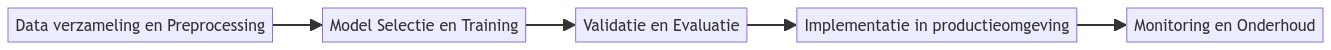
\includegraphics[width=\linewidth]{graphics/mlcycle.png}
    \caption{Machine Learning cycle}
    \label{fig:ML_cycle}
\end{figure}

Aldus \textcite{Schlegel2022} omvat de levenscyclus van een typisch Machine Learning-project verschillende fasen zoals in figuur \ref{fig:ML_cycle}:

\begin{itemize}
    \item \textbf{Data Verzameling en Preprocessing:} gegevens worden verzameld en voorbereid voor het trainen van een model, inclusief het reinigen van deze gegevens, dit word gedaan door middels van het verwerken van ontbrekende waarden en het transformeren van gegevens naar een geschikt formaat voor Machine Learning-modellen.

    \item \textbf{Model Selectie en Training:} er word een geschikt Machine Learning-model wordt geselecteerd op basis van de gegevens en het gekozen doel. Het model wordt getraind met behulp van verzamelde data, waarbij parameters worden veranderd om een zo optimaal mogelijk resultaat te bereiken.
    
    \item \textbf{Validatie en Evaluatie:} het getrainde model wordt gevalideerd met behulp van verschillende validatieset om de prestaties op nieuwe data te beoordelen.
    
    \item \textbf{Implementatie:} het model wordt geïmplementeerd om voorspellingen te genereren op data, bijvoorbeeld door integratie in een softwareapplicatie of gegevensstroom van een organisatie.

    \item \textbf{Monitoring en Onderhoud:} het model wordt continu gemonitord om de prestatie van het model over tijd te kunnen bijhouden. Indien nodig wordt het model opnieuw getraind met nieuwe data of met andere parameters om de prestaties te behouden of te verbeteren.
\end{itemize}

\subsection{Machine Learning Methoden}

Dit hoofdstuk richt zich op de verschillende onderdelen binnen het domein van Machine Learning (ML) die worden gebruikt om modellen te trainen en voorspellingen te genereren op basis van data. Aan de hand van onderzoeksvragen worden de belangrijkste methoden binnen ML uitgelegd, waarbij de nadruk ligt op het begrijpen van hun toepassingen en werking.

\begin{figure}[h]
    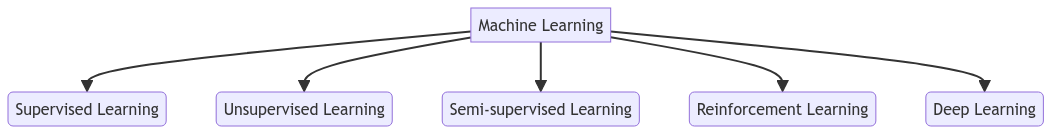
\includegraphics[width=\linewidth]{graphics/mm.png}
    \caption{Machine Learning en de subsets ervan}
    \label{fig:ML_subsets}
\end{figure}

Aldus \textcite{Mahesh2019} zijn verschillende soorten Machine Learning-methoden, waaronder:

\begin{itemize}
    \item Supervised Learning, waarbij het model wordt getraind op een dataset met gelabelde voorbeelden om een model te ontwikkelen voor nieuwe, niet eerder geziene data.

    \item Unsupervised Learning, waarbij het model wordt getraind op een dataset zonder gelabelde voorbeelden, om patronen en structuren in de data te ontdekken zonder voorafgaande kennis van de uitvoer.

    \item Semi-supervised Learning, die een combinatie van gelabelde en ongelabelde gegevens gebruikt voor training, om nauwkeuriger voorspellingen te maken.

    \item Reinforcement Learning, waarbij het model leert door interactie met een dynamische omgeving, om een optimale strategie te ontwikkelen om beloningen te maximaliseren.

    \item Deep Learning, een subset van Machine Learning die gebruikmaakt van kunstmatige neurale netwerken met meerdere lagen van verwerkingseenheden om complexe patronen in grote datasets te leren en te begrijpen.
\end{itemize}

figuur \ref*{fig:ML_subsets} visualiseert deze soorten machine learning methoden.

Machine Learning speelt een cruciale rol in het genereren van inzichten uit gegevens en het maken van voorspellingen op basis van complexe patronen \autocite{Jordan2015}. Door de levenscyclus van Machine Learning te begrijpen en verschillende soorten Machine Learning-methoden te onderzoeken, kunnen onderzoekers en ontwikkelaars effectievere en nauwkeurigere modellen ontwikkelen om een breed scala aan problemen op te lossen in bepaalde sectoren.
%%%%%%%%%%%%%%%%%%%%%%%%%%%%%%%%%%%%%%%%%%%%%%%%%%%%%%%%%%%%%%%%%%%%%%%%%%%%%%%%%%%%%%%%%%%%%%%%%%%%%%%%%%%%%%%%%%
\section{CI/CD pipelines}
%hier
Een Continuous Integration/Continuous Deployment (CI/CD) pipeline is een belangerijk onderdeel van softwareontwikkeling. Het versnelt en verbetert de levering van webapplicaties. Een CI/CD pipeline bestaat uit een opeenvolging van een reeks stappen die codewijzigingen automatisch integreren, testen en implementeren. Deze stappen omvatten Continuous Integration, Continuous Testing, Continuous Delivery en Continuous Deployment.

Dit is CI/CD pipelines uitgelegd zoals beschreven in \textcite{NaveenVemuri2024}:

Continuous Integration omvat het samenvoegen en testen van wijzegingen van diverse ontwikkelaars om ervoor te zorgen dat de verschillende delen van de code goed samenwerken en conflicten worden vermeden.

Continuous Testing houdt in dat tests automatisch worden uitgevoerd om de functionaliteit en kwaliteit van de code te controleren en evalueren. Dit zorgt ervoor dat eventuele fouten worden opgespoord voordat de code verder wordt verwerkt.

Vervolgens komt Continuous Delivery, waar de code die eerder werd getest wordt voorbereid voor implementatie in de productieomgeving. Dit omvat vaak het compileren van de code en het aaanpassen van eventuele configuratiebestanden.

Tenslotte is er Continuous Deployment, waar de voorbereide code automatisch wordt uitgevoerd in de productieomgeving. Dit minimaliseert handmatige tussenkomst en verzekert een snelle en consistente implementatie van nieuwe code.\newline

\begin{figure}[h]
    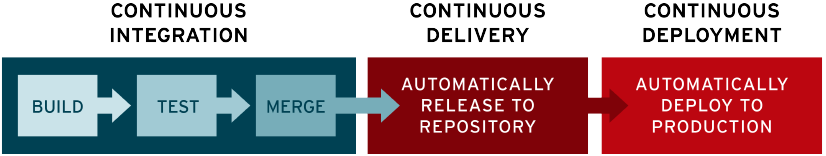
\includegraphics[width=\linewidth]{graphics/cdci.png}
    \caption{CI/CD Flow van \autocite{RedHat2023}}
    \label{fig:CICD_flow}
\end{figure}
  
Figuur \ref{fig:CICD_flow} toont de flow van een CI/CD pipeline.

Binnen het domein van datamanagement benadrukken \textcite{Samad2018} en \textcite{Vadavalasa2020} de cruciale aspecten van het optimaliseren van beperkte datasets en de implementatie van Continuous Integration in de datapipeline. Ze tonen aan dat CI/CD pipelines een belangerijke rol speelt bij het ontwikkelen van ML-modellen en en het behouden van een veilige datastroom.

CI/CD pipelines zijn een belangerijk onderdeel van softwareontwikkeling. Ze versnellen de levering van software, verhogen de kwaliteit, betrouwbaarheid en bevorderen de samenwerking tussen teams. Datapipelines spelen een cruciale rol in ML door dataverwerking te automatiseren en de efficiëntie van modeltraining te verhogen en te vereenvoudigen.
%%%%%%%%%%%%%%%%%%%%%%%%%%%%%%%%%%%%%%%%%%%%%%%%%%%%%%%%%%%%%%%%%%%%%%%%%%%%%%%%%%%%%%%%%%%%%%%%%%%%%%%%%%%%%%%%%%
\section{Machine Learning Pipelines}

Het proces van het ontwikkelen van ML-modellen omvat een complexe reeks stappen, van het verzamelen en voorbereiden van data tot het trainen, evalueren en implementeren van modellen. Deze stappen zijn vaak repetitief en tijdrovend, wat de efficiëntie en schaalbaarheid van ML-projecten kan belemmeren.

Machine Learning pipelines zijn geautomatiseerde workflows die zijn ontworpen om deze stappen in de levenscyclus van een ML-project te stroomlijnen en te automatiseren. Ze bestaan uit een reeks geordende taken, zoals data-ingestion, data-preprocessing, feature engineering, modeltraining, modelbeoordeling en modelimplementatie. Deze pipelines zorgen voor consistente en gestructureerde uitvoering van deze taken, waardoor de ontwikkeling en implementatie van ML-modellen efficiënter worden.

De voordelen van Machine Learning pipelines zijn talrijk. Ten eerste verhogen ze de efficiëntie door repetitieve taken te automatiseren, waardoor de doorlooptijd van ML-projecten wordt verkort. Bovendien zorgen pipelines voor verbeterde reproduceerbaarheid, doordat ze garanderen dat experimenten op een consistente manier worden uitgevoerd, wat essentieel is voor wetenschappelijke validatie en het delen van resultaten. Verder bieden pipelines een betere schaalbaarheid door de implementatie van ML-modellen op grotere datasets en in productieomgevingen te vergemakkelijken. Ten slotte vergroten ze de transparantie van het ML-proces door de stappen in de workflow te documenteren en te volgen.

Pipelines kunnen worden geïmplementeerd met behulp van verschillende tools en frameworks, zoals Apache Airflow, Kubeflow, Kedro, MLflow, luigi en prefect. Deze technologieën bieden een gevarieerd scala aan mogelijkheden om de ontwikkeling en implementatie van pipelines te faciliteren en te optimaliseren, afhankelijk van de specifieke behoeften en vereisten van een project.

Al met al bieden Machine Learning pipelines een efficiënte en schaalbare manier om ML-modellen te ontwikkelen en te implementeren, waardoor de reproduceerbaarheid, transparantie en efficiëntie van ML-projecten worden bevorderd.

%%%%%%%%%%%%%%%%%%%%%%%%%%%%%%%%%%%%%%%%%%%%%%%%%%%%%%%%%%%%%%%%%%%%%%%%%%%%%%%%%%%%%%%%%%%%%%%%%%%%%%%%%%%%%%%%%%
\section{Frameworks}

Machine Learning pipelines zijn een cruciaal onderdeel van het Machine Learning proces \autocite{Jordan2015}. Ze automatiseren de stappen van dataverzameling en -voorbereiding tot modeltraining en -evaluatie, waardoor het efficiënter en reproduceerbaarder wordt.

Traditioneel worden Machine Learning pipelines uitgevoerd op cloudplatforms of op krachtige servers. Dit kan echter kostbaar zijn en vereist gespecialiseerde kennis. Lokale uitvoering van Machine Learning pipelines biedt een aantal voordelen:

\begin{itemize}
  \item Lagere kosten: Lokale uitvoering maakt gebruik van de eigen hardware van de gebruiker, wat de kosten van cloudresources kan besparen.
  \item Flexibiliteit: Gebruikers hebben meer flexibiliteit om te experimenteren met verschillende frameworks en configuraties.
\end{itemize}

Deze literatuurstudie onderzoekt de verschillende frameworks die beschikbaar zijn voor het lokaal uitvoeren van Machine Learning pipelines. We bespreken de voor- en nadelen van elk framework en geven richtlijnen voor het kiezen van het juiste framework voor deze onderzoeksvraag.
\subsection{Kedro}

\textcite{Kedro2024} is een open source Python-bibliotheek die de ontwikkeling van betrouwbare, reproduceerbare en onderhoudbare Machine Learning-pipelines vereenvoudigt. Dit framework biedt een krachtige oplossing voor onderzoekers die lokaal uitgevoerde ML-pipelines willen opzetten en beheren.

Kedro biedt verschillende pluspunten waaronder:

\begin{itemize}
    \item \textbf{Flexibiliteit:} Kedro maakt het mogelijk om ML-pipelines op een flexibele manier samen te stellen. Onderzoekers kunnen eenvoudig componenten toevoegen, verwijderen of aanpassen, waardoor ze zich kunnen aanpassen aan de veranderende behoeften van hun onderzoek.
    \item \textbf{Versiebeheer:} Kedro integreert versiebeheer in ML-pipelines, waardoor experimenten reproduceerbaar worden en resultaten gevalideerd kunnen worden. Dit is cruciaal voor het bevorderen van transparantie en betrouwbaarheid in onderzoek.
    \item \textbf{Gegevenscatalogus:} Kedro biedt een geïntegreerde gegevenscatalogus waarmee onderzoekers datasets eenvoudig kunnen beheren, documenteren en traceren binnen de ML-pipeline. Dit vereenvoudigt het gegevensbeheer en bevordert de samenwerking tussen teamleden.
    \item \textbf{Lokale uitvoering:} Kedro ondersteunt lokale uitvoering van ML-pipelines, waardoor onderzoekers offline experimenten kunnen uitvoeren en ontwikkelen. Dit is met name gunstig voor onderzoek met gevoelige data of in situaties waar cloudresources niet beschikbaar zijn.
    \item \textbf{Integratie met ML-frameworks:} Kedro integreert naadloos met populaire ML-frameworks zoals TensorFlow, PyTorch en scikit-learn. Hierdoor kunnen onderzoekers hun favoriete tools blijven gebruiken binnen de Kedro pipeline.
    \item \textbf{Automatische documentatie:} Kedro kan automatisch gedetailleerde documentatie genereren voor ML-pipelines, inclusief informatie over datasets, parameters en dependencies aan de hand van de geschreven code.
    \item \textbf{Visualisatie:} Kedro biedt de mogelijkheid voor het visualiseren van ML-pipelines, waardoor er een beter begrip gekregen kan worden van de gegevensstroom en de interacties tussen verschillende componenten.
\end{itemize}

Kedro heeft vele functionaliteiten maar er zijn enkele opmerkingen waarmee rekening moet gehouden worden:

\begin{itemize}
    \item \textbf{Leercurve:} Kedro heeft een hoge leercurve, hoewel de integratie met populaire ML-frameworks dit vereenvoudigt.
    \item \textbf{Opslagruimte:} Lokale uitvoering van ML-pipelines kan, afhankelijk van de datasetgrootte, veel opslagruimte vereisen.
\end{itemize}

% TODO: bedoel je de cloud met dat laatste puntje hier?
% TODO: kan het eenvoudig vertaald worden naar bv. k8s?
Kedro is een krachtig framework voor onderzoekers die lokaal uitgevoerde ML-pipelines willen opzetten en beheren. De flexibiliteit, ondersteuning voor versiebeheer, geïntegreerde gegevenscatalogus en compatibiliteit met populaire ML-frameworks maken Kedro tot een waardevolle tool voor het lokaal uitvoeren van Machine Learning pipelines.

De volgende code is een Machine Learning-pipelines in Kedro: 

\begin{minted}[frame=lines,breaklines, linenos]{python}
    from kedro.pipeline import Pipeline, node
    from kedro.pipeline import node
    from sklearn.model_selection import train_test_split
    from sklearn.ensemble import RandomForestClassifier
    from sklearn.metrics import accuracy_score
    import pandas as pd

    def load_data():
        return pd.read_csv("data.csv")

    def split_data(data):
        X = data.drop("target", axis=1)
        y = data["target"]
        return train_test_split(X, y, test_size=0.2, random_state=42)

    def train_model(X_train, X_test, y_train, y_test):
        model = RandomForestClassifier()
        model.fit(X_train, y_train)
        return model

    def evaluate_model(model, X_test, y_test):
        preds = model.predict(X_test)
        accuracy = accuracy_score(y_test, preds)
        print("Accuracy:", accuracy)

    pipeline = Pipeline([
        node(load_data, None, "data"),
        node(split_data, "data", ["X_train", "X_test", "y_train", "y_test"]),
        node(train_model, ["X_train", "X_test", "y_train", "y_test"], "model"),
        node(evaluate_model, ["model", "X_test", "y_test"], None),
    ])
\end{minted}
%%%%%%%%%%%%%%%%%%%%%%%%%%%%%%%%%%%%%%%%%%%%%%%%%%%%%%%%%%%%%%%%%%%%%%%%%%%%%%%%%%%%%%%%%%%%%%%%%%%%%%%%%%%%%%%%%%
\subsection{MLflow}

\textcite{MLflow2023} is een open source Python bibliotheek ontwikkeld door Databricks die een uitgebreide set functionaliteiten biedt voor het beheren van Machine Learning (ML) projecten. De vier pijlers van MLflow zijn Tracking, Projects, Models en Registry:

\begin{itemize}
    \item \textbf{Tracking:} MLflow Tracking biedt een eenvoudige manier om experimenten te volgen en resultaten te vergelijken. Het registreert nauwkeurig relevante details gedurende de ML-levenscyclus, zoals code, parameters, metrieken en artefacten (modellen, datasets). Dit maakt het voor onderzoekers naadloos mogelijk om eerdere experimenten te reproduceren en verschillende configuraties te vergelijken.
    \item \textbf{Projects:} MLflow Projects zorgt voor een uniforme structuur voor ML-projecten en bevordert herbruikbaarheid. Onderzoekers kunnen gestandaardiseerde projectstructuren definiëren met MLflow Projects, waardoor consistente en reproduceerbare onderzoeksomgevingen worden gecreëerd.
    \item \textbf{Models:} MLflow Models biedt tools om modellen te verpakken en te implementeren in verschillende omgevingen. Het stroomlijnt de implementatie van ML-modellen in productieomgevingen door ze te verpakken in een gestandaardiseerd formaat, inclusief de modelcode, afhankelijkheden en configuratiedetails.
    \item \textbf{Registry:} MLflow Registry fungeert als een centrale hub voor het beheren van modelversies. Het stelt onderzoekers in staat om een gecentraliseerd repository in te stellen voor geregistreerde modellen, waardoor ze verschillende versies van modellen kunnen organiseren, volgen en openen.
\end{itemize}

% TODO: "bezig houden" klinkt negatief, zoek een beter verwoording :) je gebruikt dit nog hieronder!

MLflow biedt verschillende voordelen voor onderzoekers die zich bezighouden met ML-projecten:

\begin{itemize}
    \item \textbf{Verbeterde reproduceerbaarheid:} De zorgvuldige logging- en trackingmogelijkheden van MLflow garanderen dat experimenten gemakkelijk reproduceerbaar zijn, wat de geloofwaardigheid en betrouwbaarheid van onderzoek versterkt.
    \item \textbf{Gestroomlijnde samenwerking:} Gecentraliseerd model- en experimentbeheer bevordert naadloze samenwerking tussen onderzoekers, doordat ze elkaars werk eenvoudig kunnen delen en volgen.
    \item \textbf{Verbeterde efficiëntie:} MLflow automatiseert tijdrovende taken zoals experimenttracking en modelbeheer, waardoor onderzoekers waardevolle tijd kunnen vrijmaken voor kernonderzoeksactiviteiten.
    \item \textbf{Vereenvoudigde implementatie:} MLflow stroomlijnt het implementatieproces, waardoor onderzoekers hun modellen snel en efficiënt kunnen overbrengen van onderzoek naar productieomgevingen.
\end{itemize}

Er zijn enkele mogelijke nadelen verbonden aan het gebruik van MLflow voor het lokaal uitvoeren van Machine Learning pipelines:

\begin{itemize}
    \item \textbf{Complexiteit:} MLflow kan complex zijn om te installeren en te configureren, vooral voor onderzoekers die niet bekend zijn met Python of Databricks.
    \item \textbf{Vereist kennis:} MLflow vereist kennis van zowel Machine Learning als Python.
    \item \textbf{Beperkte integratie:} De integratie van MLflow met lokale tools en infrastructuur kan beperkt zijn.
    \item \textbf{Opslagruimte:} Het lokaal opslaan van alle experimentgegevens en artefacten kan veel opslagruimte vereisen.
\end{itemize}
MLflow is een waardevolle tool voor onderzoekers die zich bezighouden met ML-projecten. Door reproduceerbaarheid te bevorderen, samenwerking te verbeteren en experimentatie, implementatie en beheer te stroomlijnen, stelt MLflow onderzoekers in staat om de kwaliteit en efficiëntie van hun onderzoeksinspanningen te verhogen.

De volgende code is een voorbeeld van een Machine Learning pipeline in MLFlow:

% TODO: bespreek deze code ook!

\begin{minted}[frame=lines,breaklines, linenos]{python}
    import mlflow
    import mlflow.sklearn
    from sklearn.model_selection import train_test_split
    from sklearn.ensemble import RandomForestClassifier
    from sklearn.metrics import accuracy_score
    import pandas as pd
    
    def train():
        data = pd.read_csv("data.csv")
        X = data.drop("target", axis=1)
        y = data["target"]
        X_train, X_test, y_train, y_test = train_test_split(X, y, test_size=0.2, random_state=42)
        model = RandomForestClassifier()
        model.fit(X_train, y_train)
        preds = model.predict(X_test)
        accuracy = accuracy_score(y_test, preds)
        
        mlflow.log_metric("accuracy", accuracy)
        mlflow.sklearn.log_model(model, "model")
    
    if __name__ == "__main__":
        train()
\end{minted}
Deze code is een normale code voor het maken van een Machine Learning pipeline, echter zijn er enkele verschillen aangezien dat MLflow gebruikt word.
In de code kan ``log\_metrics'' en ``log\_model'' te zien zijn, deze zorgen ervoor dat bepaalde metrics te zien zijn bij de resultaten alsook dat het model word bijgehouden.
%%%%%%%%%%%%%%%%%%%%%%%%%%%%%%%%%%%%%%%%%%%%%%%%%%%%%%%%%%%%%%%%%%%%%%%%%%%%%%%%%%%%%%%%%%%%%%%%%%%%%%%%%%%%%%%%%%
\subsection{Kubeflow}
\autocite{Kubeflow2021} is een open source Machine Learning-toolkit die is ontworpen voor Kubernetes. Het biedt een krachtige infrastructuur voor onderzoekers om Machine Learning-pipelines op te zetten en te beheren in zowel lokale als cloudomgevingen.
Kubeflow biedt verschillende voordelen voor onderzoekers die zich bezighouden met het opzetten en beheren van Machine Learning-pipelines:
\begin{itemize}
    \item \textbf{Schaalbaarheid:} Door gebruik te maken van Kubernetes kan Kubeflow ML-workloads eenvoudig schalen, wat onderzoekers in staat stelt om snel te reageren op veranderende behoeften in hun onderzoek.
    \item \textbf{Geautomatiseerd beheer:} Kubeflow automatiseert de implementatie en het beheer van ML-pipelines, waardoor onderzoekers minder tijd hoeven te besteden aan handmatige configuratie en monitoring van infrastructuur, en zich meer kunnen richten op hun onderzoek.
    \item \textbf{Reproduceerbaarheid:} Met Kubeflow kunnen onderzoekers de omgeving vastleggen en de code versiebeheren, waardoor ze experimenten kunnen reproduceren en resultaten kunnen valideren, wat essentieel is voor de wetenschappelijke integriteit.
    \item \textbf{Flexibiliteit:} Kubeflow ondersteunt een breed scala aan ML-workloads, waardoor onderzoekers flexibel kunnen experimenteren met verschillende modellen en technieken binnen dezelfde infrastructuur, wat de innovatie stimuleert.
    \item \textbf{Integratie met Kubernetes:} Kubeflow is ontworpen om naadloos te integreren met Kubernetes, waardoor onderzoekers het gemakkelijk kunnen implementeren en beheren op lokale Kubernetes-clusters, wat de operationele efficiëntie verbetert.
    \item \textbf{Integratie met ML-frameworks:} Kubeflow biedt integratie met populaire ML-frameworks zoals TensorFlow, PyTorch en scikit-learn, waardoor onderzoekers hun favoriete tools kunnen blijven gebruiken binnen de Kubeflow-pipeline.
    \item \textbf{Monitoring:} Kubeflow biedt functionaliteiten voor het bijhouden en monitoren van ML-experimenten, waardoor onderzoekers inzicht krijgen in de prestaties van hun modellen en het gedrag van hun systemen kunnen volgen.
    \item \textbf{Model deployment:} Kubeflow ondersteunt model deployment en serving, waardoor onderzoekers hun modellen gemakkelijk kunnen delen en gebruiken in productieomgevingen.
\end{itemize}
Hoewel Kubeflow vele voordelen biedt, zijn er ook enkele potentiële nadelen waar onderzoekers rekening mee moeten houden:
\begin{itemize}
    \item \textbf{Complexiteit:} Kubeflow kan complex zijn om te installeren en te configureren, vooral voor onderzoekers die niet bekend zijn met Kubernetes, wat extra leer- en implementatietijd kan vereisen.
    \item \textbf{Vereist kennis:} Het effectief gebruik van Kubeflow vereist kennis van zowel Machine Learning als Kubernetes, wat een uitdaging kan zijn voor onderzoekers zonder ervaring in deze gebieden.
    \item \textbf{Beperkte ondersteuning:} De ondersteuning voor lokale uitvoering van Kubeflow is beperkter dan voor cloudomgevingen, wat mogelijk beperkingen kan opleggen aan onderzoekers die afhankelijk zijn van lokale resources.
\end{itemize}
Ondanks de mogelijke nadelen blijft Kubeflow een waardevol framework voor onderzoekers die schaalbare en flexibele ML-pipelines willen opzetten en beheren in lokale omgevingen. De voordelen zoals schaalbaarheid, geautomatiseerd beheer, ondersteuning voor reproduceerbare experimenten en integratie met populaire ML-frameworks maken Kubeflow tot een belangrijk instrument voor onderzoeksinspanningen.

De volgende code is een voorbeeld van een Machine Learning pipeline in Kubeflow:

\begin{minted}[frame=lines,breaklines, linenos]{python}
    import kfp.v2 as kfp
    from kfp.v2 import dsl
    from kfp.v2.dsl import ContainerOp, pipeline
    import pandas as pd
    from sklearn.metrics import accuracy_score
    @dsl.pipeline_op(name="data_preprocessing")
    def preprocess_data(data_path: str) -> kfp.v2.dsl.OutputArgument[pd.DataFrame]:

        data = pd.read_csv(data_path)
        X = data.drop("target", axis=1)
        y = data["target"]
        return X, y

        @dsl.pipeline_op(name="train_model")
        def train(X_train: pd.DataFrame, y_train: pd.DataFrame) -> kfp.v2.dsl.OutputArgument[RandomForestClassifier]:

        from sklearn.ensemble import RandomForestClassifier

        model = RandomForestClassifier()
        model.fit(X_train, y_train)
        return model

    @dsl.pipeline_op(name="evaluate_model")
    def evaluate(model: RandomForestClassifier, X_test: pd.DataFrame, y_test: pd.DataFrame) -> kfp.v2.dsl.OutputArgument[float]:


        preds = model.predict(X_test)
        accuracy = accuracy_score(y_test, preds)
        return accuracy

    @pipeline(name="train_rf_pipeline")
    def train_rf_pipeline(data_path: str):

    X_train, y_train = preprocess_data(data_path)

    model = train(X_train, y_train)

    accuracy = evaluate(model, X_train.copy(), y_train.copy())

    kfp.compiler.Compiler().compile(train_rf_pipeline, package_path="pipeline.yaml")
\end{minted}

%%%%%%%%%%%%%%%%%%%%%%%%%%%%%%%%%%%%%%%%%%%%%%%%%%%%%%%%%%%%%%%%%%%%%%%%%%%%%%%%%%%%%%%%%%%%%%%%%%%%%%%%%%%%%%%%%%
\subsection{ZenML}

\textcite{ZenML2024} is een open-source framework voor het definiëren en beheren van Python-gebaseerde Machine Learning (ML) pipelines. Het biedt een end-to-end oplossing voor het ontwikkelen, implementeren en beheren van dergelijke pipelines, met als doel de complexiteit van het ML-levenscyclus te vereenvoudigen.

Belangrijke Kenmerken van ZenML:
\begin{itemize}
    \item \textbf{Geïntegreerde pipeline-opslag:} ZenML biedt een centrale repository voor het opslaan van pipelines, waardoor hergebruik en delen eenvoudig worden gemaakt.
    \item \textbf{Lokale en op afstand uitvoering:} Pipelines kunnen zowel lokaal als op afstand worden uitgevoerd, met ondersteuning voor verschillende platforms zoals Kubernetes en Docker.
    \item \textbf{Uitgebreide monitoring:} ZenML biedt uitgebreide monitoringfunctionaliteit om de voortgang en prestaties van pipelines nauwkeurig te volgen.
    \item \textbf{Efficiënt herstarten:} Pipelines kunnen efficiënt worden herstart vanaf een mislukte stap, wat de foutopsporing vereenvoudigt en versnelt.
    \item \textbf{MLOps-integratie:} ZenML integreert MLOps-functionaliteit, inclusief artefactbeheer, versiebeheer en experimentenbeheer, waardoor het aantrekkelijk is voor teams die streven naar best practices op het gebied van Machine Learning operations.
    \item \textbf{Gebruiksvriendelijkheid:} ZenML heeft een eenvoudige leercurve en is flexibel in configuratie en aanpassing.
    \item \textbf{Breed scala aan functionaliteiten:} ZenML biedt een breed scala aan functionaliteiten om aan de diverse behoeften van ML-projecten te voldoen.
\end{itemize}

Voordelen van ZenML in vergelijking met andere frameworks:
\begin{itemize}
    \item \textbf{Eenvoudiger leercurve:} ZenML heeft een eenvoudiger leercurve dan andere frameworks zoals Apache Airflow, Luigi en Kubeflow Pipelines.
    \item \textbf{Flexibeler:} ZenML biedt meer flexibiliteit in configuratie en aanpassing dan andere frameworks.
    \item \textbf{Breder scala aan functionaliteiten:} ZenML biedt een breder scala aan functionaliteiten dan andere frameworks, inclusief expliciete focus op MLOps.
\end{itemize}
ZenML is een framework dat zich richt op gebruiksvriendelijkheid, schaalbaarheid en het implementeren van MLOps-best practices. Het is een waardevolle aanwinst voor onderzoeksgemeenschappen en industriële toepassingen, en biedt data scientists en Machine Learning engineers een krachtige tool voor het beheren van ML pipelines.

De volgende code is een voorbeeld van een Machine Learning pipeline in ZenML:

\begin{minted}[frame=lines,breaklines, linenos]{python}
    from sklearn.model_selection import train_test_split
    from sklearn.ensemble import RandomForestClassifier
    from sklearn.metrics import accuracy_score
    import pandas as pd
    @step
    def read_data():
        data = pd.read_csv("data.csv")
        X = data.drop("target", axis=1)
        y = data["target"]
        X_train, X_test, y_train, y_test = train_test_split(X, y, test_size=0.2, random_state=42)

    @step    
    def train():
        model = RandomForestClassifier()
        model.fit(X_train, y_train)
        preds = model.predict(X_test)
        accuracy = accuracy_score(y_test, preds)
    
    @pipeline
    def main():
        train(read_data())

    if __name__ == "__main__":
        run = main()
\end{minted}
In deze code maakt ZenML gebruik van decorators, deze decorators zijn:
\begin{itemize}
    \item \textbf{@step:} Deze decorator word voor elke functie geplaats die moet worden uitgevoerd worden als een taak, een taak is een onderdeel van een pipeline.
    \item \textbf{@pipeline:} Deze decorator gaat alle functies met de step decorator uitvoeren, deze decorator kan ook meerde opties bevatten zoals het gebruiken van cache. Deze cache zorgt ervoor dat een al uitgevoerde step niet opnieuw word uitgevoerd als er geen verandering is.
\end{itemize}

Deze code heeft dus 2 steps die dan samen in de pipeline worden uitgevoerd. Eerst word de read\_data() uitgevoerd die dan zijn resultaten naar de functie train stuur om het model te trainen.
%%%%%%%%%%%%%%%%%%%%%%%%%%%%%%%%%%%%%%%%%%%%%%%%%%%%%%%%%%%%%%%%%%%%%%%%%%%%%%%%%%%%%%%%%%%%%%%%%%%%%%%%%%%%%%%%%%
\subsection{Prefect}

\textcite{Prefect2024} is een open-source framework voor het beheren van Python-gebaseerde Machine Learning (ML) pipelines. Het maakt gebruik van gerichte acyclische grafieken (DAG's) om de stappen in de pipeline en hun onderlinge afhankelijkheden expliciet te definiëren. Prefect biedt een breed scala aan functies voor het beheren en uitvoeren van pipelines, waaronder opslag, uitvoering, monitoring en het herstarten van pipelines vanaf een mislukte stap.

Voordelen van Prefect voor het lokaal uitvoeren van ML pipelines:

\begin{itemize}
  \item \textbf{interface:} Prefect biedt een gebruiksvriendelijke interface voor het volgen van de pipeline uitvoeringen en de resultaten hiervan.
  \item \textbf{Schaalbaarheid:} Prefect is schaalbaar en kan pipelines uitvoeren op verschillende platforms, dit kan lokaal maar ook in de cloud zoals, AWS of Azure.
  \item \textbf{Flexibiliteit:} Prefect is flexibel configureerbaar om aan de specifieke behoeften van elk project te voldoen.
  \item \textbf{Uitgebreide functies:} Prefect biedt een breed scala aan functies voor het beheren en uitvoeren van pipelines.
\end{itemize}

In vergelijking met andere frameworks voor het beheren van ML pipelines, zoals Apache Airflow, Luigi, Kubeflow Pipelines enzovoort, onderscheidt Prefect zich door:

\begin{itemize}
  \item \textbf{Gebruiksvriendelijkheid:} Prefect heeft een eenvoudigere leercurve en een duidelijke interface.
  \item \textbf{Flexibiliteit:} Prefect is gemakkelijker aan te passen aan de specifieke behoeften van een project.
  \item \textbf{Uitgebreide functies:} Prefect biedt meer functies dan sommige concurrenten.
\end{itemize}
\begin{minted}[frame=lines,breaklines, linenos]{python}
\end{minted}
Prefect is een gebruiksvriendelijk framework voor het beheren en uitvoeren van ML pipelines. Met zijn schaalbaarheid, flexibiliteit en uitgebreide functieset is Prefect een uitstekende keuze voor data scientists en Machine Learning engineers die op zoek zijn naar een betrouwbare oplossing voor het beheren van hun ML workflows.

% \subsection{Dagster}
% \textcite{Dagster2024} is een open-source framework voor het beheren en uitvoeren van Machine Learning (ML) pipelines. Het maakt gebruik van een modulaire structuur en heeft een focus op operationele efficiëntie. Dagster is snel aan het groeien door de flexibiliteit en schaalbaarheid.

% Voordelen van Dagster voor het lokaal uitvoeren van ML pipelines:
% \begin{itemize}
%     \item Modulair: Dagster heeft een modulaire architectuur dat het maken, onderhouden en hergebruiken van pipelines vereenvoudigt. Elke onderdeel kan worden gecombineerd om een workflow te maken.
%     \item Efficiëntie: Dagster legt de focus op efficiëntie, waardoor dat alle onderliggend technologieën de pipeline niet zou vertragen.
%     \item MLOps: Dagster integreert MLOps-best practices, onderandere versie-, experimentenbeheer en artifacts managment voor het beheren van pipelines. Dit maakt het makkelijker 
%     \item Schaalbaarheid: Dagster kan worden gebruikt om pipelines uit te voeren op een lokale machine, op clusters of in de cloud.
% \end{itemize}
% Ondanks alle voordelen bied Dagster ook enkele nadelen:
% \begin{itemize}
%     \item Nieuw: Dagster is relatief nieuw en heeft nog geen uitgebreide documentatie, community en integraties met andere frameworks.
%     \item Leercurve: Dagster is modulair dit kan het moeilijker maken om te begrijpen en te implementeren, zeker voor mensen die dit soort syntax niet gewoon zijn. Door de leercurve kan het ontwikkelen van pipelines langer duren.
%     \item Klein eocsysteem: Dagster zijn ecosteem is nog steeds in ontwikkeling, hierdoor heeft dagster niet alle integraties en componenten dat andere frameworks bieden.
% \end{itemize}
% Dagster is een goede keus voor het beheren van ML-pipelines. De modulaire architectuur en de vele functies voor het maken van pipelines maken het een goede keuze voor onderzoekers, data scientists en ontwikkelaars die Machine Learning pipelines willen ontwikkelen. Dagster is wel relatief nieuw waardoor het niet alle functionaliteiten heeft die andere frameworks wel hebben.

\subsection{Luigi}

Luigi is een open-source Python-bibliotheek die een krachtige en gebruiksvriendelijke oplossing biedt voor het uitvoeren van complexe Machine Learning (ML) pipelines op een schaalbare manier. Het kernconcept van Luigi draait om het definiëren van workflows als gerichte acyclische grafieken (DAG's), waarbij elke taak in de grafiek afhankelijk kan zijn van andere taken. Deze aanpak maakt het eenvoudig om pipelines te maken die bestaan uit een groot aantal afzonderlijke stappen.

Voordelen van Luigi:
\begin{itemize}
  \item Gebruiksgemak: Luigi is ontworpen met gebruiksgemak in gedachten, waardoor het eenvoudig is om pipelines te definiëren en te configureren.
  \item Schaalbaarheid: Luigi kan draaien op clusters van machines en taken automatisch parallel uitvoeren, waardoor het workflows kan schalen naar grote datasets.
  \item Betrouwbaarheid: Luigi heeft functionaliteit om fouten te verwerken, zoals het automatisch opnieuw uitvoeren van mislukte taken en het herstellen van workflows.
  \item Flexibiliteit: Luigi is geschikt voor zowel grootschalige implementaties als lokale uitvoeringen van ML-pipelines.
\end{itemize}

Waarom Luigi niet kiezen voor ML-pipelines:
\begin{itemize}
    \item Complexiteit: Hoewel Luigi gebruiksvriendelijker is dan sommige andere frameworks, kan het nog steeds complex zijn om te implementeren en te configureren, vooral voor beginners. Dit kan de leercurve verhogen en de tijd die nodig is om pipelines op te zetten verlengen.
    \item Beperkte integratie: Luigi heeft mogelijk niet dezelfde mate van integratie met andere ML-tools en -bibliotheken als andere frameworks, wat kan leiden tot extra handmatig werk en complexiteit.
    \item Beperkte flexibiliteit: Luigi's DAG-gebaseerde structuur kan beperkend zijn voor complexe pipelines met onregelmatige of dynamische workflows. In dergelijke scenario's kunnen andere frameworks meer flexibiliteit en aanpassingsmogelijkheden bieden.
  \end{itemize}

Luigi is een krachtige en gebruiksvriendelijke oplossing voor het uitvoeren van ML-pipelines. De voordelen van Luigi, zoals gebruiksgemak, schaalbaarheid, betrouwbaarheid en flexibiliteit, maken het een aantrekkelijke keuze voor onderzoekers, data scientists en ontwikkelaars die ML-workflows willen beheren en implementeren.
\begin{minted}[frame=lines,breaklines, linenos]{python}
\end{minted}
%%%% Apache Airflow: https://airflow.apache.org/
%%Luigi: https://luigi.readthedocs.io/en/stable/
%%%Kubeflow Pipelines: https://www.kubeflow.org/docs/pipelines/
%%% GITHUB PREFECT EN PREFECT DOCS BRON


\section{Requirementsanalyse}

Om te bepalen welk framework gebruikt zal worden, werd in samenwerking met de copromotor een lijst van requirements opgesteld. Deze lijst omvat alle criteria die een framework moet hebben om te worden gebruikt in het opleidingsonderdeel ``Machine Learning Operations''.

% TODO: kijk eens naar sectie 2.12 en verder van https://thesis.hogent.be/2022-2023/1330_202075027_PBA-TIN_scriptie.pdf om te zien hoe je deze sectie het best aanpakt

De risicoanalyse bestaat uit twee delen: de ``must-haves'' en de ``should-haves''. De "must-haves" zijn criteria waaraan het framework absoluut moet voldoen. De ``should-haves'' omvatten de eigenschappen die wenselijk zijn voor een framework, maar niet essentieel zijn.

De must haves zijn:
\begin{itemize}
    \item De pipeline moet op eender welk besturingssysteem uitvoerbaar zijn (Windows, macOS en Linux)
    \item De omgeving waarin de pipeline uitgevoerd wordt is reproduceerbaar
    \item De pipeline moet uitvoerbaar zijn op een toestel dat voldoet aan de minimumvereisten van de opleiding
    \item De concepten van de pipeline kunnen vertaald worden naar een cloud omgeving (bv. Azure ML)
    \item De pipeline wordt beschreven in een leesbaar formaat (bv. YAML)
    \item De pipeline is in staat om lokaal uitgevoerd te worden, al dan niet met een minimalistisch model
\end{itemize}
De should haves zijn:
\begin{itemize}
    \item De pipeline kan in een container uitgevoerd worden
    \item De pipeline kan een rollback uitvoeren wanneer het model niet voldoet aan vooropgestelde criteria
\end{itemize}

Aan de hand van deze criteria zal besloten worden welke framework(s) gekozen zal worden om de Proof-of-Concept uit te werken.

\begin{landscape}
    \begin{table}[]
    \begin{tabular}{lllllll}
    Criteria                                                               & Kedro                                                               & Luigi                                                              & Prefect                                                           & \begin{tabular}[c]{@{}l@{}}Apache \\ Airflow\end{tabular}         & ZenML                                                             & Kubeflow                                                          \\
    OS compatibiliteit                                                     & \begin{tabular}[c]{@{}l@{}}Windows, \\ macOS, \\ Linux\end{tabular} & \begin{tabular}[c]{@{}l@{}}Windows, \\ macOS,\\ Linux\end{tabular} & \begin{tabular}[c]{@{}l@{}}Windows,\\ macOS,\\ Linux\end{tabular} & \begin{tabular}[c]{@{}l@{}}Windows,\\ macOS,\\ Linux\end{tabular} & \begin{tabular}[c]{@{}l@{}}Windows,\\ macOS,\\ Linux\end{tabular} & \begin{tabular}[c]{@{}l@{}}Windows,\\ macOS,\\ Linux\end{tabular} \\
    Reproduceerbaarheid                                                    & Ja                                                                  & Ja                                                                 & Ja                                                                & Ja                                                                & Ja                                                                & Ja                                                                \\
    Minimumvereisten                                                       & Ja                                                                  & Ja                                                                 & Ja                                                                & Ja                                                                & Ja                                                                & Ja                                                                \\
    \begin{tabular}[c]{@{}l@{}}Cloud\\ compatibiliteit\end{tabular}        & Ja                                                                  & Ja                                                                 & Ja                                                                & Ja                                                                & Ja                                                                & Ja                                                                \\
    \begin{tabular}[c]{@{}l@{}}Leesbaar\\ formaat\end{tabular}             & YAML                                                                & Python code                                                        & Python code                                                       & \begin{tabular}[c]{@{}l@{}}DAGs \\ (Python code)\end{tabular}     & YAML                                                              & \begin{tabular}[c]{@{}l@{}}YAML\\ en Python \\ code\end{tabular}  \\
    Lokale uitvoering                                                      & Ja                                                                  & Ja                                                                 & Ja                                                                & Ja                                                                & Ja                                                                & Ja                                                                \\
    \begin{tabular}[c]{@{}l@{}}Data verzamelen\\ en verwerken\end{tabular} & Ja                                                                  & Ja                                                                 & Ja                                                                & Ja                                                                & Ja                                                                & Ja                                                                \\
    \begin{tabular}[c]{@{}l@{}}Model trainen\\ en evalueren\end{tabular}   & Ja                                                                  & Ja                                                                 & Ja                                                                & Ja                                                                & Ja                                                                & Ja                                                                \\
    Model deployen                                                         & Ja                                                                  & Ja                                                                 & Ja                                                                & Ja                                                                & Ja                                                                & Ja                                                               
    \end{tabular}
    \end{table}
    \end{landscape}